\subsubsection{Theory Overview}
\label{subseq:direct-sparse methods}

Direct sparse methods combine the main advantages of direct and iterative methods. In other words, numerical accuracy of the methods is comparable with the standard Gaussian Elimination process while their computational complexity is typically bounded by $O(n^2)$ \cite{complexity-of-spdm} due to treatment of non-zero matrix elements. As it is in case of direct dense methods, a solution of a system of equations is computed by means of forward and backward substitutions using $LU$ decomposition of the corresponding matrix.\\


A multi-frontal method is probably the most representative example of direct sparse solvers, inroduced by \citeauthor{mult-frontal-original:1} in work \cite{mult-frontal-original:1}. The method is, in fact, an improved version of the frontal method \cite{frontal-original} and can compute independent fronts in parallel. A front, also called a frontal matrix, can be considered as a small dense matrix resulting from a column elimination of the original system. There also exist left- and right-looking vatiants of the multi-frontal method explained in detail in \cite{elimination-tree}.\\


In this subsection, the theory of multi-frontal method is explained, which helps to understand parallel aspects and strong scaling behavior of   direct sparse solvers in case of parallel execution. To keep the overview rather simple, we assume matrix $A$ is real, symmetric and sparse. In this case, $LU$ decomposition of matrix $A$ boils down to Cholesky factorization \ref{eq:chol-1}.\\

\begin{equation} \label{eq:chol-1}
	A = LDL^T
\end{equation}

The algorithm starts with symbolic factorization of system \ref{eq:chol-1} with the aim of predicting of sparsity pattern of factor $L$. Once it is done the corresponding elimination tree can be constructed.\\

\figpointer{\ref{fig:sparsity-pattern-example-mm}}

\begin{figure}[htpb]
  \centering
  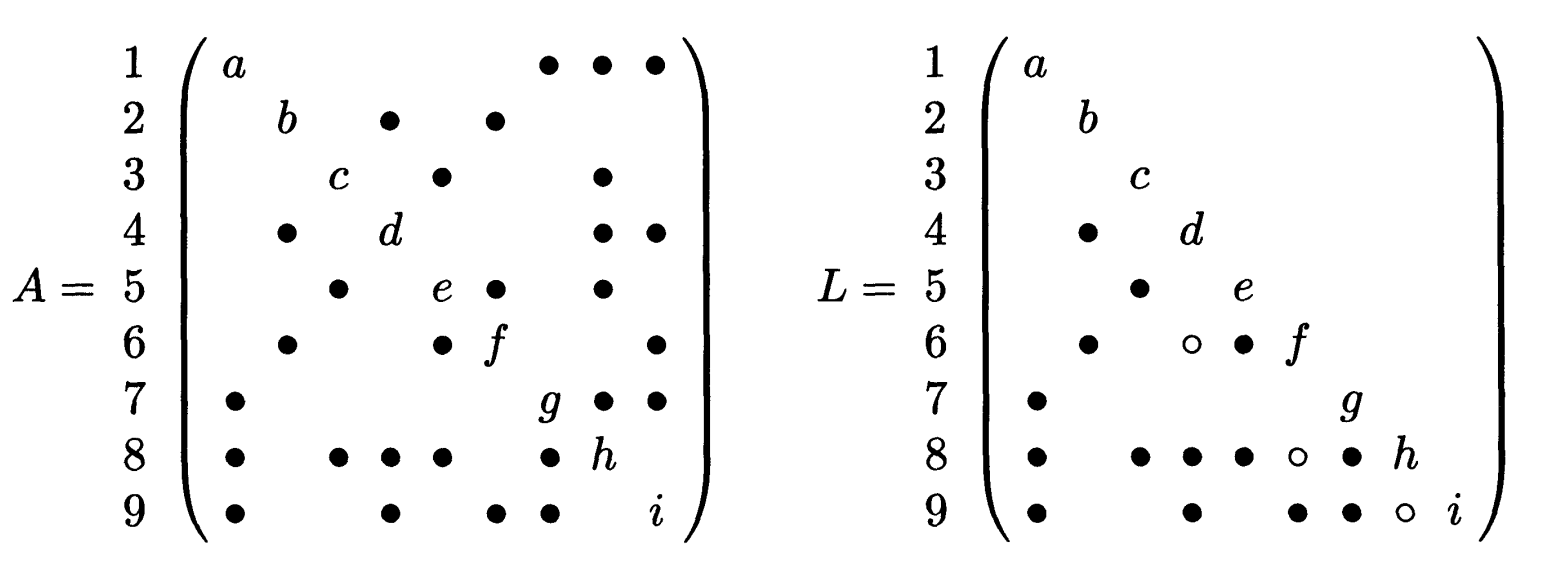
\includegraphics[width=0.9\textwidth]{figures/chapter-2/sparsity-pattern-example-mm.png}
\caption{An example of a sparse matrix and its Cholesky factor \cite{mult-frontal-original:2}}
\label{fig:sparsity-pattern-example-mm}
\end{figure}


Figure \ref{fig:sparsity-pattern-example-mm} shows an illustrative example of a sparse matrix $A$ and its Cholesky factor $L$ taking from \cite{mult-frontal-original:2}. The solid circles represent original non-zero elements whereas hollow ones define fill-in factors of $L$. \\


The elimination tree is a crucial part of the method. It can be considered as a structure of $n$ nodes where node $p$ is the parent of $j$ if and only if it satisfies equation \ref{eq:elimination-tree-1}. It is worth pointing out the definition \ref{eq:elimination-tree-1} is not only one possible and one can define a strucutre of the elimination tree in a different way as well, \cite{mult-frontal-original:2}.\\% As an example, another definition of an ellimination tree, alos refered as an assembly tree, was defined by \citeauthor{mult-frontal-original:2} in \cite{mult-frontal-original:2}.\\

\begin{equation} \label{eq:elimination-tree-1}
	p = min(i > j | l_{ij} \neq 0)
\end{equation}


In fact, node $p$ represents elimination of the corresponding column $p$ of matrix $A$ as well as all dependencies of column $p$ factorization on results of eliminations of its descendants.\\


Given definition \ref{eq:elimination-tree-1} and a sparsity pattern of factor $L$, the corresponding elimination tree can be constructed, as it is shown in figure \ref{fig:elimination-tree-mm}.\\


\figpointer{\ref{fig:elimination-tree-mm}}

\begin{figure}[htpb]
  \centering
  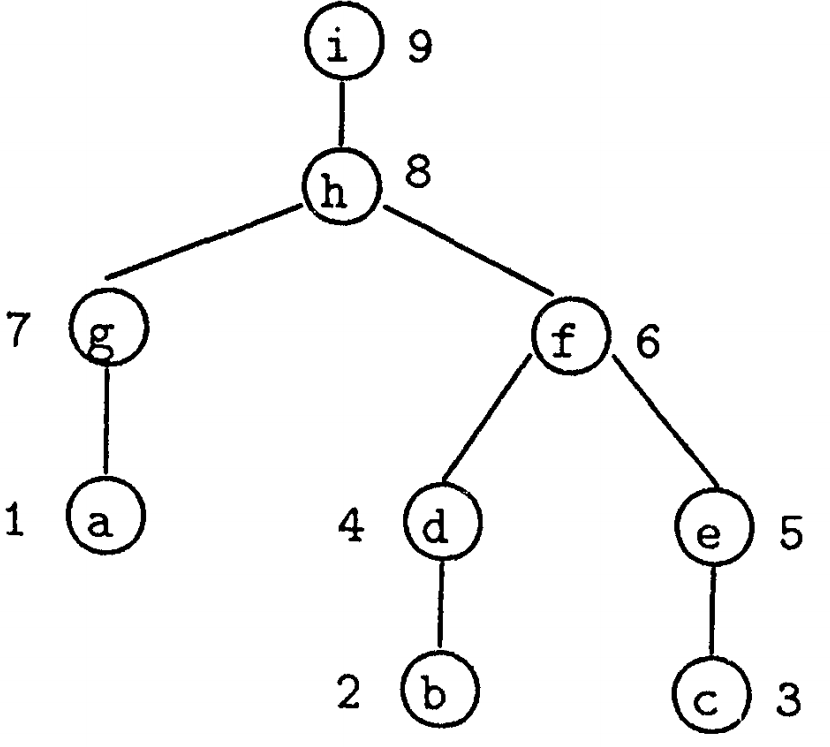
\includegraphics[width=0.45\textwidth]{figures/chapter-2/elimination-tree-mm.png}
\caption{An elimination tree of matrix $A$ from example depicted in figure \ref{fig:sparsity-pattern-example-mm}
 \cite{mult-frontal-original:2}}
\label{fig:elimination-tree-mm}
\end{figure}


The fundamental idea of multi-frontal method spins around frontal and update matrices. Frontal matrix $F_{j}$ is used to perform Gaussian Elimination for a specific column $j$ and it is equal to a sum of  frame $Fr_{j}$ and update $\hat{U_{j}}$ matrices, as it can be observed from equation \ref{eq:mm-1}\\.

\begin{equation} \label{eq:mm-1}
	F_{j} = Fr_{j} + \hat{U_{j}} = \begin{bmatrix}a_{j,j} & a_{j,i_1} & a_{j,i_2} & \dots & a_{j,i_r} \\
a_{i_1,j} \\
a_{i_1,j} \\
\vdots & & & 0\\
a_{i_r,j} \\
\end{bmatrix} + \hat{U_{j}}
\end{equation}

where $i_{0}$, $i_{1}$, \dots , $i_{r}$ are row subscripts of non-zeros in $L_{*j}$ where $i_{0} = j$; $r$ is the number of off-diagonal non-zero elements.\\

Frame matrix $Fr_{j}$ is filed with zeros except the first row and column which contain non-zero elements of the $j$th row and column of the original matrix $A$. Because of symmetry of matrix $A$, the frame matrix is square and symmetric.\\

In order to describe parts of an elimination tree, notation $T[j]$ is introduced to represent all descendants of node $j$ in the tree and node $j$ itself. In this case, update matrix $\hat{U_{j}}$ can be defined as follows:\\

\begin{equation} \label{eq:mm-2}
	\hat{U_{j}} = - \sum_{k \in T[j] -{j}}  \begin{bmatrix}
l_{j,k} \\
l_{i_1,k} \\
\vdots \\
l_{i_1,k} \\
\end{bmatrix} \begin{bmatrix}
l_{j,k} & l_{i_1,k} & \dots & l_{i_1,k}
\end{bmatrix} 
\end{equation}


Update matrix $\hat{U_{j}}$ is, in fact, can be considered as the second term of the Schur complement i.e. update contributions from already factorized columns of $A$.\\

The subscript $k$ represents descendant columns of node $j$. Hence, only those elements of descendant columns are included and considered which correspond to the non-zero pattern of the $j$th column.\\

Let's consider a partial factorization of 2-by-2 block dense matrix, equation \ref{eq:mm-3}, to better understand the essence of update matrix $\hat{U_{j}}$. Let's assume that  matrix $B$ has already been factorized and can be expressed as follows: \\


\begin{equation} \label{eq:mm-4}
	B = L_{B}L^{T}_{B}
\end{equation}


\begin{equation} \label{eq:mm-3}
A = \begin{bmatrix}
B & V^{T} \\
V & C
\end{bmatrix} 
= 
\begin{bmatrix}
L_{B} & 0 \\
VL^{-T}_{B} & I
\end{bmatrix}
\begin{bmatrix}
I & 0 \\
0 & C - VB^{-1}V^{T}
\end{bmatrix} 
\begin{bmatrix}
L^{T}_{B} & L^{-1}_{B}V^{T} \\
0 & I
\end{bmatrix} 
\end{equation}


The Schur complement, from equation \ref{eq:mm-3}, can be viewed as a sum of the original sub-matrix $C$ and update $-VB^{-1}V^{T}$. The update matrix can be written in a vector form as follows:

\begin{equation} \label{eq:mm-5}
	-VB^{-1}V^{T} = -(VL^{-T}_{B})(L^{-1}_{B}V^{T}) = - \sum_{k=1}^{j-1}  \begin{bmatrix}
l_{j,k} \\
\vdots \\
l_{n,k} \\
\end{bmatrix} \begin{bmatrix}
l_{j,k} & \dots & l_{n,k}
\end{bmatrix} 
\end{equation}

Firstly, it can be clearly observed that equations \ref{eq:mm-5} and \ref{eq:mm-2} are similar. However, equation \ref{eq:mm-2} exploits sparsity of the corresponding rows and columns of factor $L$ and, therefore, masks unnecessary information. Secondly, frame matrix $Fr_{j}$ corresponds to block matrix $C$ and brings information from the original matrix $A$. At the same time, update matrix $\hat{U_{j}}$ adds information about the columns that have already been factorized.\\

% both eqautions show that the update matrix aggregate all previous information done and in case of the ,ultifrontal methods it means that we aggregate all information from descendants

% Therefore, we can express Uy as an aggregate of outer- product updates from columns in T[Cl],..., T[cs]. 

%We can also notice from equation \ref{eq:mm-3} that the frame matrix $Fr_{j}$ corresponds to the block matrix $C$ and brings information from the original matrix $A$ whereas matrix $\hat{U_{j}}$ adds information about the columns that have already been factorized.\\

As soon as frontal matrix $F_{j}$ is assembled, i.e. the complete update of column $j$ has been computed, elimination of the first column of matrix $F_{j}$ can be started which will result in computing of non-zero entries of factor column $L_{*j}$. The process is denoted as a partial factorization of matrix $F_{j}$.\\

Let's denote $\hat{F_{j}}$ as a result of the first column elimination of frontal matrix $F_{j}$. Then, the elimination process of column $j$ can be expressed as follows:\\


\begin{equation} \label{eq:mm-6}
\hat{F_{j}} = \begin{bmatrix}
l_{j,j} & \dots & 0 \\
\vdots & I \\
l_{i_{r},j} \\
\end{bmatrix} 
\begin{bmatrix}
1 & \dots & 0 \\
\vdots & U_{j} \\
0 \\
\end{bmatrix} 
\begin{bmatrix}
l_{j,j} & \dots & l_{i_{r},j} \\
\vdots & I \\
0 \\
\end{bmatrix} 
\end{equation}

where sub-matrix $U_{j}$ represents the full update from all descendants of node $j$ and node $j$ itself. Equation \ref{eq:mm-7} expresses sub-matrix $U_{j}$ in a vector form: \todo{check formula}\\

\begin{equation} \label{eq:mm-7}
\hat{U_{j}} = - \sum_{k \in T[j]}  \begin{bmatrix}
l_{i_1,k} \\
\vdots \\
l_{i_1,k} \\
\end{bmatrix} \begin{bmatrix}
l_{i_1,k} & \dots & l_{i_1,k}
\end{bmatrix}
\end{equation}


Update column matrix $U_{j}$, also called as a contribution matrix, together with the frontal $F_{j}$ and update $\hat{U_j}$ matrices, forms the key concepts of the multi-frontal method. Let's consider an example, depicted in figure \ref{fig:information-float}, to demonstrate importance of contribution matrices.\\



\figpointer{\ref{fig:information-float}}
\begin{figure}[htpb]
  \centering
  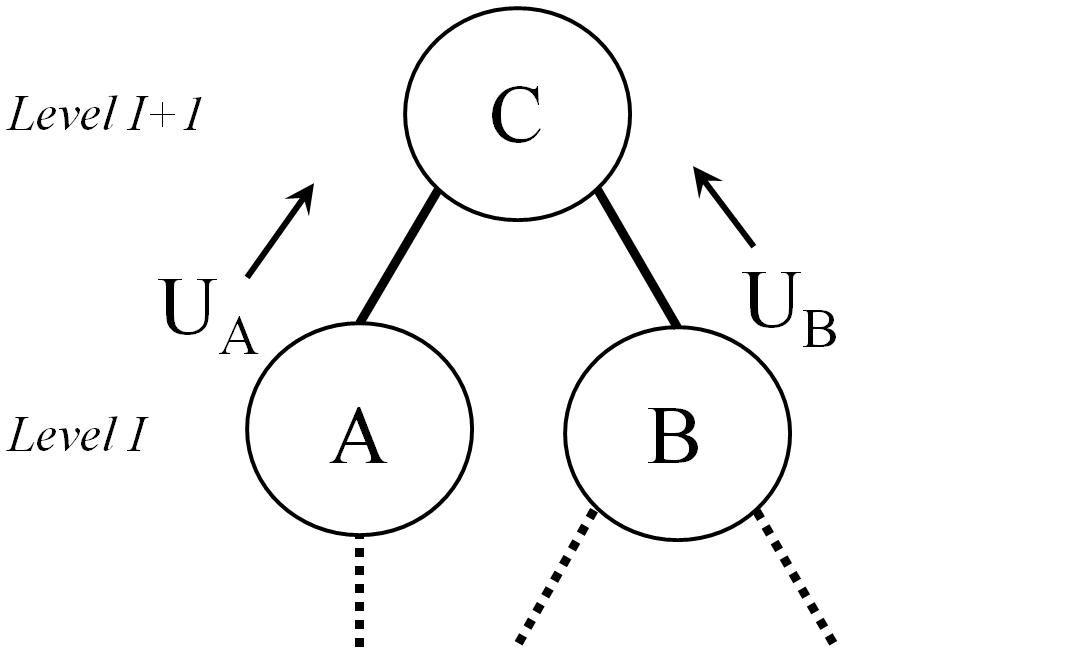
\includegraphics[width=0.45\textwidth]{figures/chapter-2/information-flow.png}
\caption{Information flow of the multifrontal method}
\label{fig:information-float}
\end{figure}


Let's assume that columns A and B have already been factorized and the corresponding contribution matrices $U_{A}$ and $U_{B}$ have already been computed. According to equation \ref{eq:mm-7}, it is known that both $U_{A}$ and $U_{B}$ matrices contain the full updates of all their descendants including updates of columns $A$ and $B$ as well. Therefore, update column matrices $U_{A}$ and $U_{B}$ have already contained all necessary information to construct update matrix $\hat{U_{C}}$. A detailed proof and careful explanation can be found in \cite{mult-frontal-original:2}.\\


It can happen that only a subset of rows and columns of matrices $U_{A}$ and $U_{B}$ is needed due to sparsity of column $C$. Hence, only relevant elements of the corresponding matrices have to be retrieved to \textit{form} matrix $\hat{U_{C}}$. For that reason, an additional matrix operation, called \textbf{\textit{extend-add}}, has be introduced in the theory of direct sparse methods.\\


%It might happen that we do not need all rows and columns of $U_{A}$ and $U_{B}$ i.e. we need only some subset of them, because of sparsity of column $C$ . It is also important to place all necessary rows and columns of matrices $U_{A}$ and $U_{B}$ in a right place within matrix $\hat{U_{C}}$. For that reason, an additional matrix operation, called \textbf{\textit{extend-add}}, must be introduced.\\

As an example, taking from \cite{mult-frontal-original:2}, let's consider the extend-add operation applied to 2-by-2 matrices $R$ and $S$ which correspond to indices ${5,8}$ and ${5,9}$ of a matrix $B$, respectively.\\

\begin{equation}
R = \begin{bmatrix}
p & q \\
u & v \\
\end{bmatrix} 
,
\:
S = \begin{bmatrix}
w & x \\
y & z \\
\end{bmatrix} 
\end{equation}

The result of such operation is a 3-by-3 matrix $K$ which can be written as follows:\\

\begin{equation} \label{eq:mm-8}
K = R \extendadd S = \begin{bmatrix}
p & q & 0 \\
u & v & 0 \\
0 & 0 & 0 \\
\end{bmatrix} 
+
\begin{bmatrix}
w & 0 & x \\
0 & 0 & 0 \\
y & 0 & z \\
\end{bmatrix} 
=
\begin{bmatrix}
p + w & q & x \\
u & v & 0 \\
y & 0 & z \\
\end{bmatrix} 
\end{equation}

Hence, formation of frontal matrix $F_{j}$ can be expressed using the extend-add operation and all direct children of node $j$ as follows:


\begin{equation} \label{eq:mm-9}
	F_{j} = \begin{bmatrix}a_{j,j} & a_{j,i_1} & a_{j,i_2} & \dots & a_{j,i_r} \\
a_{i_1,j} \\
a_{i_1,j} \\
\vdots & & & 0\\
a_{i_r,j} \\
\end{bmatrix} \extendadd U_{c_1} \extendadd \dots \extendadd U_{c_s} 
\end{equation}

where $c_{1}, \: c_{2}, \: \dots \: c_{n}$ are indices of direct children of node $j$.\\

At this point, it is worth mentioning the resulting frontal matrix $F_{j}$ forms a small dense block which has to be factorized along the first column. The partial factorization of such a block can efficiently performed by means of the corresponding dense linear algebra kernels.\\


After partial factorization of matrix $F_{j}$, assembly of contribution matrix $U_{j}$ must be completed by adding those elements of $U_{c_1}, \:, U_{c_2}, \: \dots, U_{c_s}$ to $U_{j}$ that have not been used in factorization of $F_{j}$ due to sparsity of column $j$. Then, the process continues moving up along the tree. Therefore, complete update matrices are growing in size while the global elimination process is moving towards the root of the tree.\\


Manipulations with frontal and contribution matrices play a significant role in performance of the multi-frontal method. Sometimes contribution matrices, generated in previous steps, must be stored into a temporary buffer and efficiently retrieved from it later during the global factorization process. This can require to change column elimination order which can be achieved by some matrix re-ordering thecniques. For instance, \textit{post-ordering}, mentioned by \citeauthor{mult-frontal-original:2} in \cite{mult-frontal-original:2}, can be considered as an example of such re-ordering, in case of symmetric matrices, and can eventually make efficient use of \textit{stack} data structure. Post-ordering is based on topological ordering and thus it is equivalent to the original matrix order. Hence,  such re-ordering results in the same fill-in of the factor \cite{mult-frontal-original:2}.\\


%In case of a symmetric matrix, one can apply \textit{postordering} in order to make use of \textit{stack} data structure.




%Another important aspect is storage and manipulation of frontal and contribution matrices. Sometimes we have to store contribution matrices produced in previous steps into some temporary buffer and efficiently retrieve them later during factorization. This can require some matrix re-ordering. In case of symmetric matrices, one can apply postordering on a tree to be able to use the stack data structure to alleviate the process of contribution matrix manipulations during factorization. A tree postordering is based on topological ordering and it has been proven that it is equivalent to the original matrix ordering and thus leads to the same filled graph \cite{mult-frontal-original:2}. \todo{sentence refactoring} We refer to the original matrix ordering as the ordering received from fill-in reduction operation.\\


A post-ordered tree implies that each node is ordered before its parent and nodes in each subtree are numbered consecutively. Figure \ref{fig:mm-matrix-postordering} shows an example of post-ordering applied to the elimination tree of the matrix shown in figure \ref{fig:sparsity-pattern-example-mm}. As a result, consecutive \textit{push} and \textit{pop} operations can be efficiently used during matrix factorization and thus can result in significant simplification of a computer program, see figure \ref{fig:mm-contrib-matrix-manipulation}.



%The results of this can be observed in figure \ref{fig:mm-contrib-matrix-manipulation} where consecutive \textit{push} and \textit{pop} operations are efficiently used during factorization and thus simplify the program logic.\\


\figpointer{\ref{fig:mm-matrix-postordering}}
\begin{figure}[htpb]
  \centering
  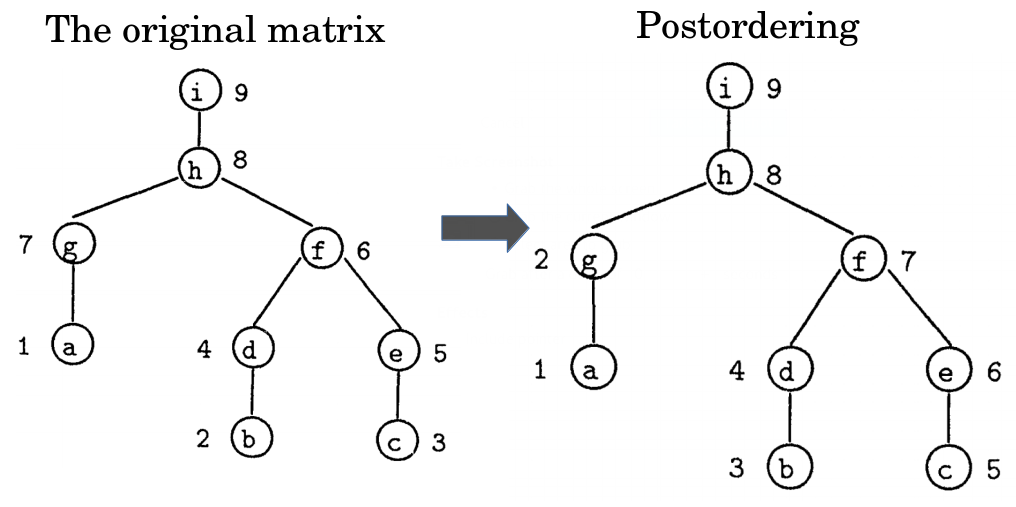
\includegraphics[width=0.75\textwidth]{figures/chapter-2/elimination-tree-mm-postordering.png}
\caption{An example of matrix postordering from \cite{mult-frontal-original:2}}
\label{fig:mm-matrix-postordering}
\end{figure}


\figpointer{\ref{fig:mm-contrib-matrix-manipulation}}
\begin{figure}[htpb]
  \centering
  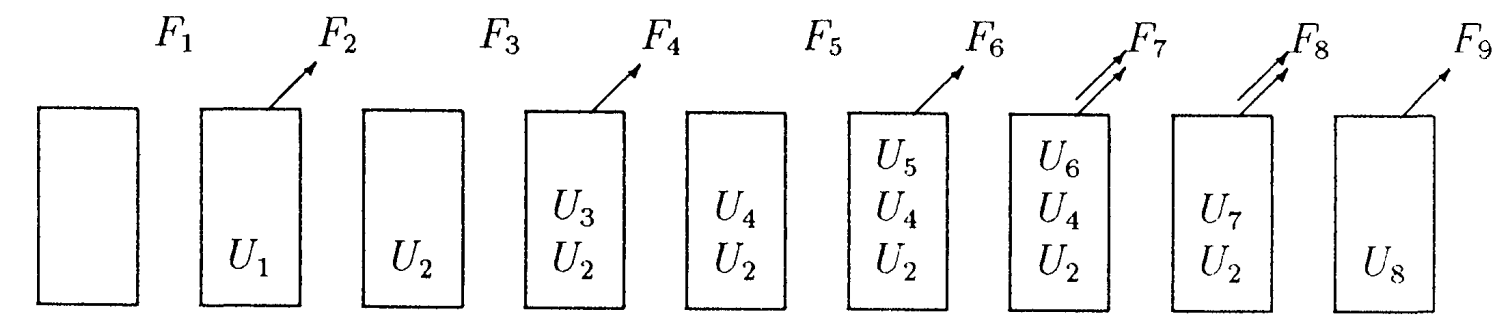
\includegraphics[width=0.75\textwidth]{figures/chapter-2/mm-contrib-matrix-manipulation.png}
\caption{The stack contents for the postordering \cite{mult-frontal-original:2}}
\label{fig:mm-contrib-matrix-manipulation}
\end{figure}


% supernodal
In practice, an improved version of multi-frontal method, called super-nodal method, is used. The method tends to shrink an elimination tree by grouping some certain nodes/columns in a single node. As a result, more floating point operations can be performed per memory access by eliminating few columns at once within the same frontal matrix.\\


% FOR PRESENTATION: Working on supernodes instead of individual variables is essential in order to speed-up the computations and use high-level BLAS [72] (Basic Linear Algebra Subprograms): supernodes lead to a higher flops to memory access ratio, and this allows a better usage of memory hierarchy and better performance thanks to the blocking techniques used in BLAS routines.



A super-node is formed by a set of contiguous columns which have identical off-diagonal sparsity structure. Hence, a super-node has two important properties. Firstly, it can be expressed as a set of consecutive column indices, namely: $\{j, \: j+1, \: \dots, \:j + t\}$ where node $j + k$ is a parent of $j + k - 1$ in the corresponding elimination tree. Secondly, the size of super-nodal frontal matrix $\mathcal{F}_{j}$ is equal to the size of frontal matrix $F_{j}$ resulted from the original post-ordered tree. As an example, figure \ref{fig:supernodal-method-postordering-and-etree} shows a post-ordered matrix $A$, its Cholesky factor $L$ and the resulting super-nodal elimination tree.\\


\figpointer{\ref{fig:supernodal-method-postordering-and-etree}}

\begin{figure}[htpb]
  \centering
  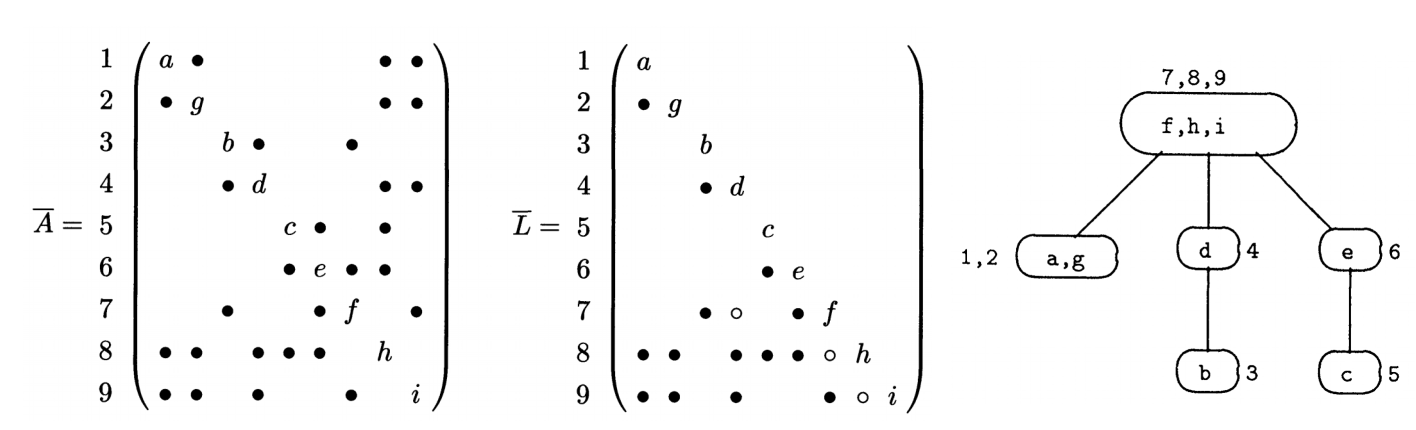
\includegraphics[width=1.0\textwidth]{figures/chapter-2/supernodal-method-postordering-and-etree.png}
\caption{An example of a supernodal elimination tree \cite{mult-frontal-original:2}}
\label{fig:supernodal-method-postordering-and-etree}
\end{figure}
 
 
Equation \ref{eq:mm-10} shows an assembly process of super-nodal frontal matrix $\mathcal{F}_{j}$. In contrast to \ref{eq:mm-9}, the frame matrix $\mathcal{F}r_{j}$ contains more dense rows and columns. As before, the \textit{extend-add} operation is used to construct the full update block from contribution matrices of children, namely: $ U_{c_1}, \:\: U_{c_2}, \:\: \dots, \:\: U_{c_s} $.\\


\begin{equation} \label{eq:mm-10-0}
	\mathcal{F}_{j} = \mathcal{F}r_{j} \extendadd U_{c_1} \extendadd \dots \extendadd U_{c_s} 
\end{equation}


 \begin{equation} \label{eq:mm-10}
	\mathcal{F}_{j} = \begin{bmatrix}a_{j,j} & a_{j,j+1} & \dots & a_{j,j+t}  & a_{j,i_1} & \dots & a_{j,i_r} \\
a_{j+1,j} & a_{j+1,j+1} & \dots & a_{j+1,j+t}  & a_{j+1,i_1} & \dots & a_{j+1,i_r} \\
\vdots & \vdots & \dots & \vdots \\
a_{j+t,j}  & a_{j+t,j+1} & \dots & a_{j+t,j+t}  & a_{j+t,i_1} & \dots & a_{j+t,i_r} \\
a_{i_1,j} & a_{i_1,j+1} & \dots & a_{i_1,j+t} \\
\vdots & \vdots & \dots & \vdots  & & 0\\ 
a_{i_r,j} & a_{i_r,j+1} & \dots & a_{i_r,j+t} \\
\end{bmatrix} \extendadd U_{c_1} \extendadd \dots \extendadd U_{c_s} 
\end{equation}


It is worth mentioning there exist other definitions of a super-node which allow to amalgamate even more nodes from the original post-ordered tree. For example, \citeauthor{mult-frontal-original:2} pointed out, in \cite{mult-frontal-original:2}, a super-node could be defined without the column contiguity constrain which can result in denser frame matrix $\mathcal{F}r_{j}$.\\


It can be clearly observed the methods consist of three distinct phases, namely: analysis, numerical factorization and solution phases. The analysis phase includes fill reducing matrix re-ordering, symbolic factorization, post-ordering, node amalgamation, elimination tree construction, estimation of required memory space etc. During the numerical factorization phase, $L$ and $D$, or $U$, factors of the original matrix $A$ are computed based on sequence of partial factorizations of frontal matrices. Given matrix decomposition, the solution step computes a solution vector $x$ by means of backward and forward substitutions.\\



\subsubsection{Parallelization Aspects}
\label{subseq:direct-parallel-aspects}


In contrast to iterative methods, parallelization of direct sparse methods mainly comes from task-based parallelism where an elimination tree can be considered as a collection of tasks. In fact, a tree represents data dependencies during column partial factorizations and, therefore, reveals dependent and independent tasks. For example, leaves usually locate in separate branches of the tree and thus represent concurrent tasks that can be executed in parallel. On the other hand, parent nodes represent data dependences from their children and cannot be factorized beforehand. Therefore, sparse direct methods have only limited parallelism which swiftly decreases while computations are moving towards the top of an elimination tree.\\


Let's consider two simple models, that have been developed for this study, in order to demonstrate potential parallel performance of tree-task parallelism. The models, in fact, are perfectly balanced binary trees with different costs per level. Within a level, the cost is distributed equally among the nodes. The first model, figure \ref{fig:mm-parallel-model-tree-linear}, implies 
quadratic decrease of computational cost between nodes of adjacent levels whereas the second one, figure \ref{fig:mm-parallel-model-tree-quadratic}, simulates cubic decay of compute-intensity. The models intend to reflect growth of complete update matrices in size, while moving from bottom to top along an elimination tree, and thus increase of floating point operations.\\




%The elimination tree, in fact, represents dependencies among columns. Conversely, the tree also shows independent steps of elimination process. Hence the tree forms independent problems that can be executed in parallel. Task parallelism is the main and primary source the algorithm parallelisation. Figure \ref{fig:elimination-tree-mm-parallel-steps} shows task parallelism, for the example given in Figure \ref{fig:supernodal-method-postordering-and-etree}, where each color represents a set concurrent tasks.\\


%\figpointer{\ref{fig:elimination-tree-mm-parallel-steps}}

%\begin{figure}[htpb]
%  \centering
%  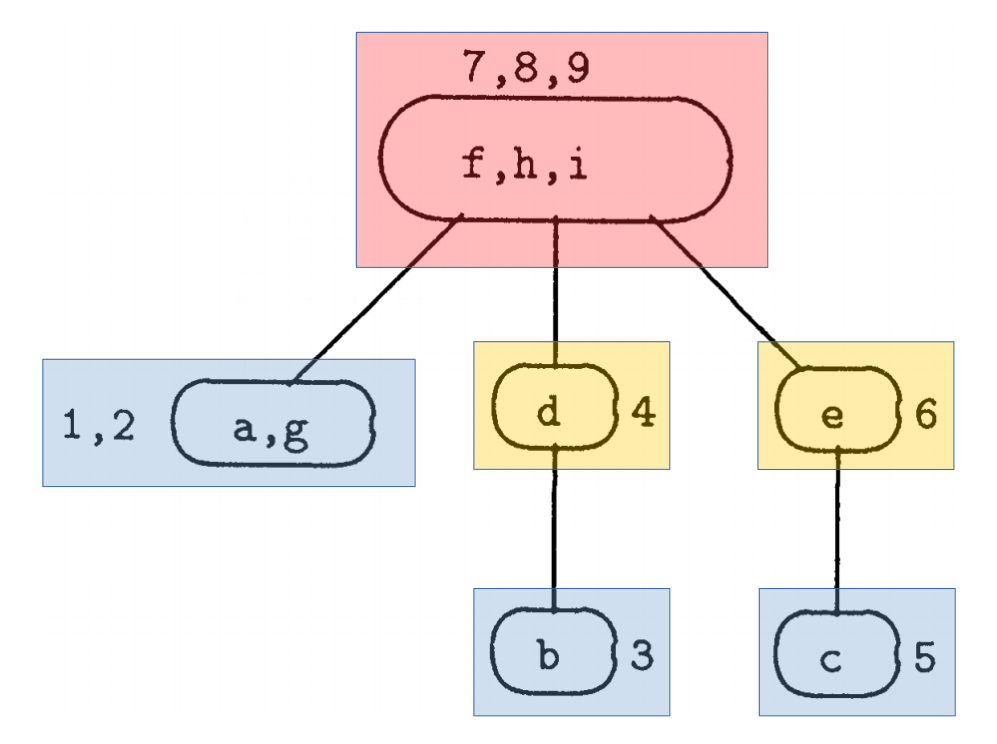
\includegraphics[width=0.5\textwidth]{figures/chapter-2/elimination-tree-parallel.png}
%\caption{Parallel steps of the multifrontal method based on the example in Figures \ref{fig:supernodal-method-postordering-and-etree}}
%\label{fig:elimination-tree-mm-parallel-steps}
%\end{figure}


%For example, nodes on separate branches of the tree are totally independent and can processed in parallel. However, as soon as at least two branches run into the same node it forms a dependency and we have to wait all contribution matrices of its children and cannot proceed further.\\ 


%We can observe the amount of task parallelism is rapidly decreasing while moving towards the root along the tree. Once we reach the root of the tree the algorithm becomes totally sequential. This fact can play the significant role in strong scaling behavior of the method.\\


%We developed two simple models based on perfectly balanced binary trees to better understand strong scaling of the algorithm. The main concept of the models is so-called cost per level or cost per node. This idea is similar to the recursion trees in \cite{recursion-tree} which explains and computes complexity of recurrent algorithms.\\


%Figure \ref{fig:mm-parallel-model-tree-linear} represents the first model where we keep the same cost per level whereas the second model (Figure \ref{fig:mm-parallel-model-tree-quadratic}) simulates quadratic cost decay from level to level. Additionally we assume that computational cost distributed uniformly between nodes at the same level for both models.\\


\figpointer{\ref{fig:mm-parallel-model-tree}}
\begin{figure}
\centering
	\begin{tabular}{cc}
			\subfloat[Model 1: equal cost per level]{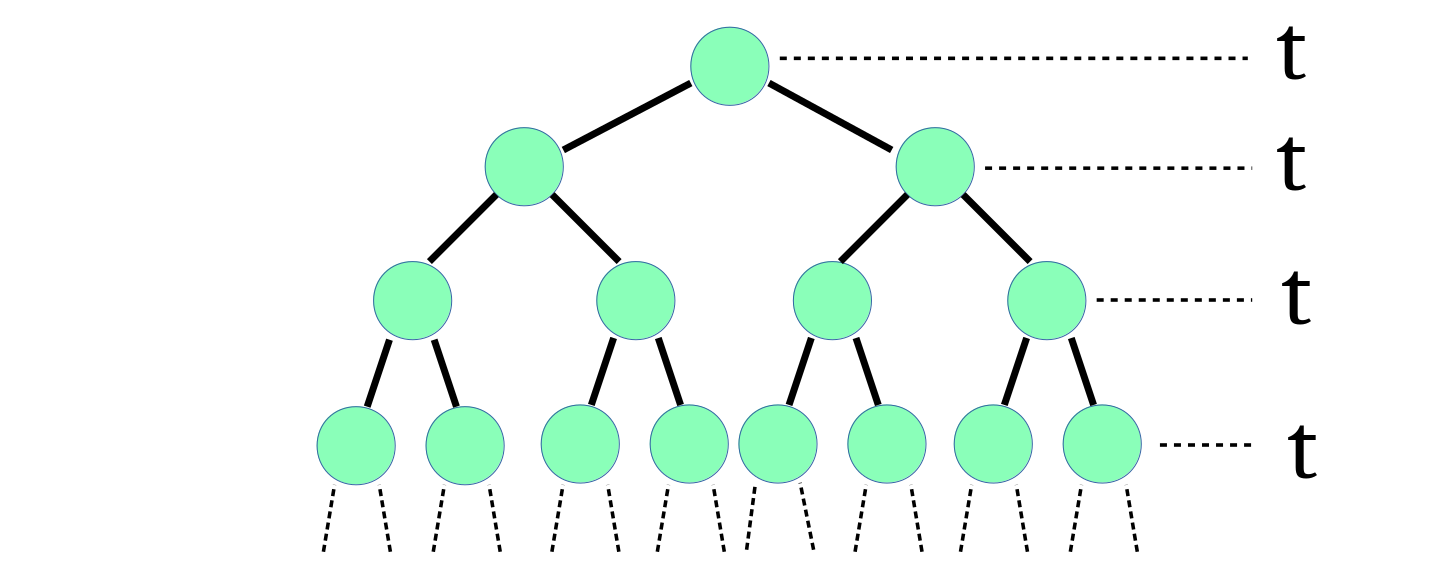
\includegraphics[width=0.5\textwidth]{figures/chapter-2/mm-parallel-model-tree-1.png} \label{fig:mm-parallel-model-tree-linear}} & 
		\subfloat[Model 2: quadratically decreasing cost per level]{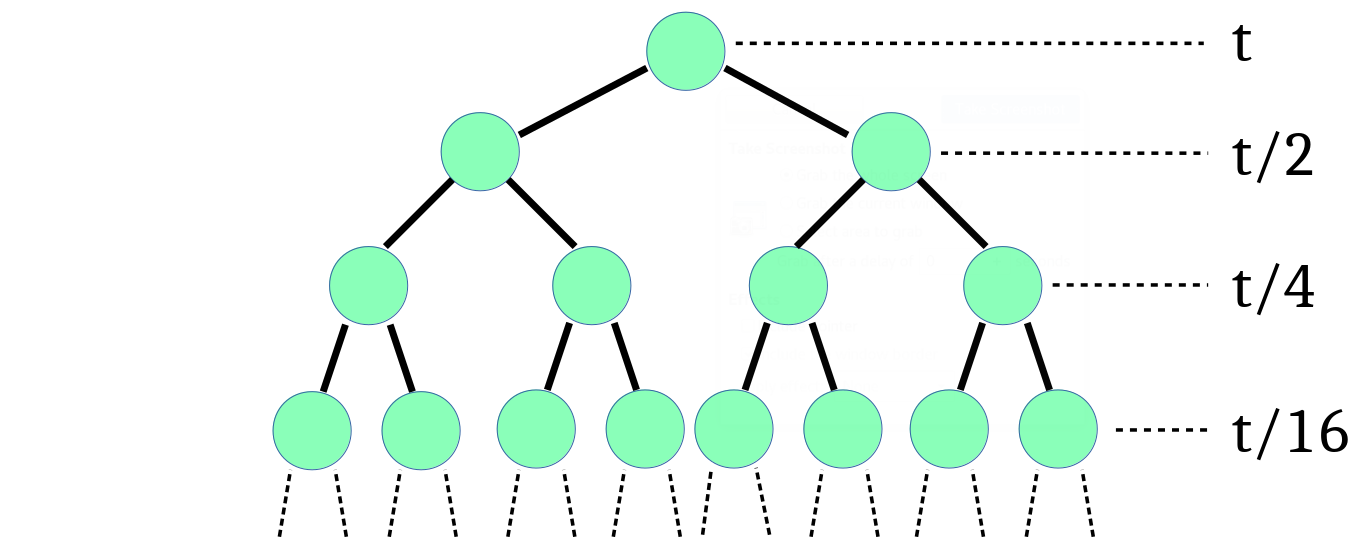
\includegraphics[width=0.5\textwidth]{figures/chapter-2/mm-parallel-model-tree-2.png} \label{fig:mm-parallel-model-tree-quadratic}} \\
	\end{tabular}
	\caption{Simple parallel models of the multifrontal method}
	\label{fig:mm-parallel-model-tree}
\end{figure}

%We have to say that our models mimic only numerical factorization and do not include time spent on any per-processing steps, for example, fill-in reduction reodering. A cost per level can be interpreted in different ways e.g. increase of partial factorization time due to growth of frontal matrices in size, time increase spent on numerical pivoting, increase of MPI communication overheads due to growth of contribution matrices, etc. It should be mentioned that real computer implementations of the multifrontal algorithm (MUMPS, SuperLU, etc.) are quite sophisticated in many aspects and our models do not have any intention to analyze performance of a particular package. Instead the objective of these models is to show possible strong scaling behavior and possible bottlenecks. \\


%We will consider only task parallelism at the beginning to a first approximation and later we will discuss how additional data parallelism can affect algorithm performance.\\

% assumtion that cost is equal within the level!!!


The models imply parallel computations within a  level but sequential execution between them. In other words, to start computations at the next top level, factorizations of all nodes at the current  one have to be fully performed. It also means that computations at the next level cannot be started  even if there are some available free processors but factorization of the last node at the current level has not been completed yet. Thereby, minimal execution time  of both models can be exactly evaluated based on the model descriptions. Essentially, it is equal to a sum of time spent on single node of each level. Therefore, it determines asymptotes on the corresponding speed-up graphs.\\

%As we mentioned above the root of the tree can be processed purely sequentially if we only consider task parallelism. As a first approximation, time spent on the root factorization determines the minimal execution time according to the Amdahl's low \cite{wiki:amdahls-low}. More precisely, the minimal execution time is equal to a sum of time spent on a single node at each level. This time determines the asymptote in the corresponding speed-up graph.\\


Figures \ref{fig:mm-parallel-model-tree-linear} and \ref{fig:mm-parallel-model-tree-quadratic} represent strong scaling behavior of both models filled with 65535 nodes i.e. 16 levels. As it can be observed, the models demonstrate a rapid drop of parallel performance, especially in case of the quadratic one, figure \ref{fig:mm-parallel-model-tree-quadratic} . Table \ref{table:mm-potential-model-speed-up} compares speed-up of two models obtained with 32768 and 20 abstract processors. Number 32768 is equal to the number of leaves at the bottom level and thus implicitly determines maximum speed-up. It is worth mentioning that two models almost exhaust tree-task parallelism even with 20 processing elements. Further increase of processor count can only barely improve the overall parallel performance.\\


\figpointer{\ref{fig:mm-parallel-model-speed-up}}
\begin{figure}
\centering
	\begin{tabular}{cc}
			\subfloat[Theoretical speed-up of Model 1]{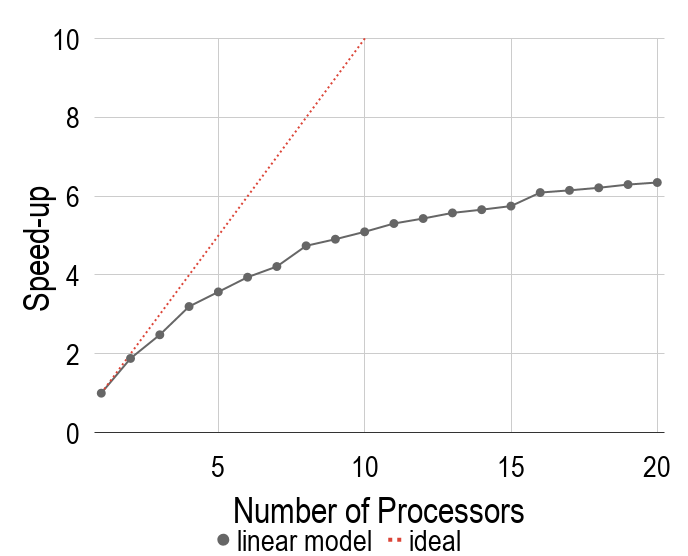
\includegraphics[width=0.45\textwidth]{figures/chapter-2/mm-parallel-model-tree-1-speedup.png}} &
		\subfloat[Theoretical speed-up of Model 2]{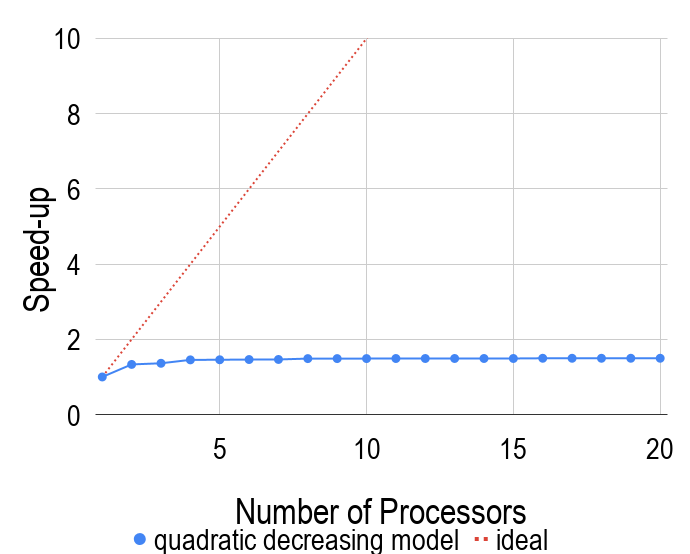
\includegraphics[width=0.45\textwidth]{figures/chapter-2/mm-parallel-model-tree-2-speedup.png}} \\
	\end{tabular}
	\caption{Theoretical speed-up}
	\label{fig:mm-parallel-model-speed-up}
\end{figure}


\begin{table}[htpb]
\centering
\small
\begin{tabular}{|c|c|c|}
\hline
        & 20 PEs  & 32768 PEs \\ \hline
Model 1 & 6.3492  & 8.0000    \\ \hline
Model 2 & 1.4972 & 1.5000   \\ \hline
\end{tabular}
\caption{Potential speed-up of linear and quadratic models}
\label{table:mm-potential-model-speed-up}
\end{table}


These, rather simple, models reveal the most important fact about tree-task parallelism of sparse direct solvers. The performance depends heavily on an elimination tree and, in particular, on distribution of compute-intensity among nodes. As it was mentioned above, the intensity is usually centered on the top part of the tree where task-based parallelism is limited due to data dependency. As an example, \citeauthor{mult-frontal-original:2} observed that factorization of the last 6 nodes took slightly more than 25\% of the total number of floating point operations in case of application of the multi-frontal method to a $k-by-k$ regular model problem using a nine-point difference operator, \cite{mult-frontal-original:2}.\\


Node-data parallelism is often combined with tree-task parallelism which usually results in improvement of parallel performance of direct sparse methods. In the general case, frontal matrix $\mathcal{F}_{j}$ can be distributed across multiple processors and partially factorized in parallel. However, because of fine granularity of bottom levels data parallelism is only applied to top  and middle parts of elimination trees.\\ 

Performance of node-data parallelism depends on  both a frontal matrix size and the number of processors assigned to perform partial factorization. For example, over-subscription of processing elements to a node can result in slow-down induced by communication overheads.\\


By and large, combined tree-task and node-data parallelism improves performance and strong scaling of sparse direct solvers, however, it cannot change the performance trend mainly induced by tree-task parallelism. Therefore, one can still expect  stagnation of speed-up even with a relatively small number of processors.\\


A parallel implementation of sparse direct solvers demands to expand the analysis phase by adding 
two more pre-processing steps, namely: process mapping and load balancing. Both mapping and balancing are usually performed statically during an analysis of an elimination tree.\\ %However, a refinement of these steps can become necessary to perform in run-time during the numerical factorization phase due to partial pivoting.\\



%Both models shows that computational intensity per node grows from bottom to top. It is easy to conclude from Figure \ref{fig:mm-parallel-model-tree} that intensity per node is equal $t/2^{i}$ and $t/2^{2i}$ for the first and second models, respectively (where $i$ is a level of the tree). It reflects that the most intensive part of the method is centered on the top part of the tree i.e. first few level. \citeauthor{mult-frontal-original:2} discussed application of the multifrontal method to a $k-by-k$ regular model problem with nine-point difference operator in his paper \cite{mult-frontal-original:2}. He observed that factorization of the last 6 nodes took slightly more than 25\% of the total amount of arithmetical operations. As a comparison, table \ref{table:mm-simple-model-work-load} shows fractions of time spent on processing first few top levels of our models: 1 and 2.\\


%\begin{table}[htpb]
%\centering
%\begin{tabular}{|c|c|c|}
%\hline
%        & Model 1 & Model 2 \\ \hline
%Level 0 & 6.25\%  & 50.00\% \\ \hline
%Level 1 & 12.50\% & 75.00\% \\ \hline
%Level 2 & 18.75\% & 87.50\% \\ \hline

%\end{tabular}
%\caption{Distribution workload per level in case model 1 and 2}
%\label{table:mm-simple-model-work-load}
%\end{table}


%By and large, reduction of time spent on the top nodes is a way to improve strong scaling behavior. To do so, data parallelism can be additionally exploited for these nodes. It is worth noting that data parallelism at bottom levels does not make sense because it leads to increase of granularity there and thus increase communication overheads which can lead to significant performance drop.\\


%Figure \ref{fig:mumps-task-data-parallelism} shows an example of two types of parallelism applied to the algorithm. First of all, we can see the leaves are grouped in subtrees and a single PE is assigned to each subtree. Other nodes are distributed among three different types. Nodes of the first type uses task parallelism only, which is induced by the tree, and each node is executed in a single processor. The second type exploits data parallelism with 1D block row distribution among the processors. The root belongs to the third type where data parallelism is used with 2D block cyclic distribution. The details of MUMPS parallelism management is carefully explained and can be found in \cite{mumps:task-data-parallelism}.\\


%\figpointer{\ref{fig:mumps-task-data-parallelism}}

%\begin{figure}[htpb]
%  \centering
%  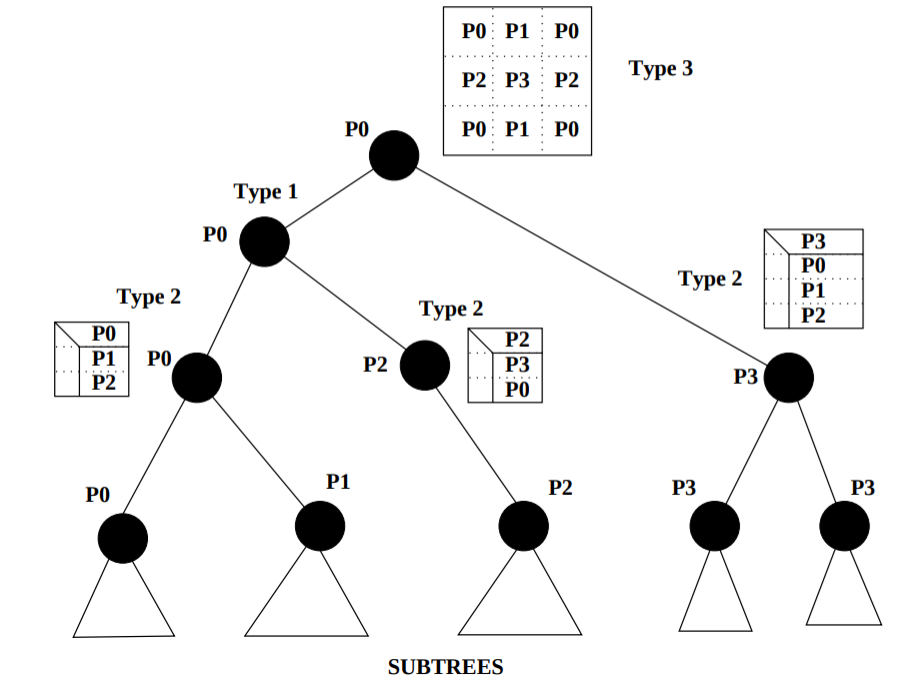
\includegraphics[width=0.65\textwidth]{figures/chapter-2/mumps-task-data-parallelism.png}
%\caption{MUMPS parallelism management in case of 4 PEs \cite{mumps:task-data-parallelism}}
%\label{fig:mumps-task-data-parallelism}
%\end{figure}


%All the techniques mentioned above were designed to improve strong scaling behavior by splitting the most intensive parts among all available processors. Going back to our models, we can also think about that in a slightly different way, namely: \textit{data parallelism helps to re-distribute cost per node/level on the corresponding elimination tree}. However, we have to notice that efficiency of data parallelism totally depends on sizes of frontal matrices at the top part of the tree. In case of skinny sparse matrices, oversubscription of processing elements can lead to strong performance penalties as we could see from section \ref{subseq:direct methods}. A machine-dependent minimal frontal matrix size was introduced in MUMPS in order to control whether to use ScaLAPACK at the root node or not \cite{mumps-manual}. It can happen that the algorithm uses only task parallelism, due to the threshold, and, as a results, scaling will only depend on the tree structure that can be deep and unbalanced.\\


%Figure \ref{fig:model-1-vs-mumps} shows comparison of strong scaling between model 1 and parallel numerical factorization of the matrix \textit{\textbf{memchip}} (Table \ref{table:suite-sparse-matrix-set}) done with using MUMPS library. The sparsity pattern before and after fill-in reduction is shown in figure \ref{fig:memchip-matrix-sparsity-pattern}. 

%\todo{add some examples to the appendix}
%\figpointer{\ref{fig:model-1-vs-mumps}. Show standard deviation}
%\begin{figure}[htpb]
%  \centering
%  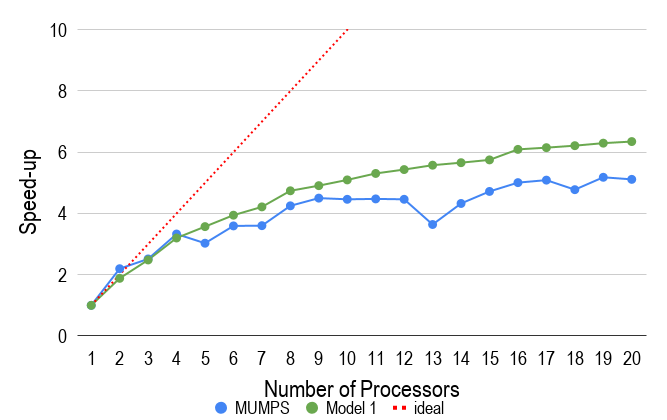
\includegraphics[width=0.65\textwidth]{figures/chapter-2/model-1-vs-mumps.png}
%\caption{Comparison between model 1 and numerical factorization of the matrix \textit{\textbf{memchip}} using MUMPS library}
%\label{fig:model-1-vs-mumps}
%\end{figure}


%\figpointer{\ref{fig:memchip-matrix-sparsity-pattern}}
%\begin{figure}[htpb]
%  \centering
%  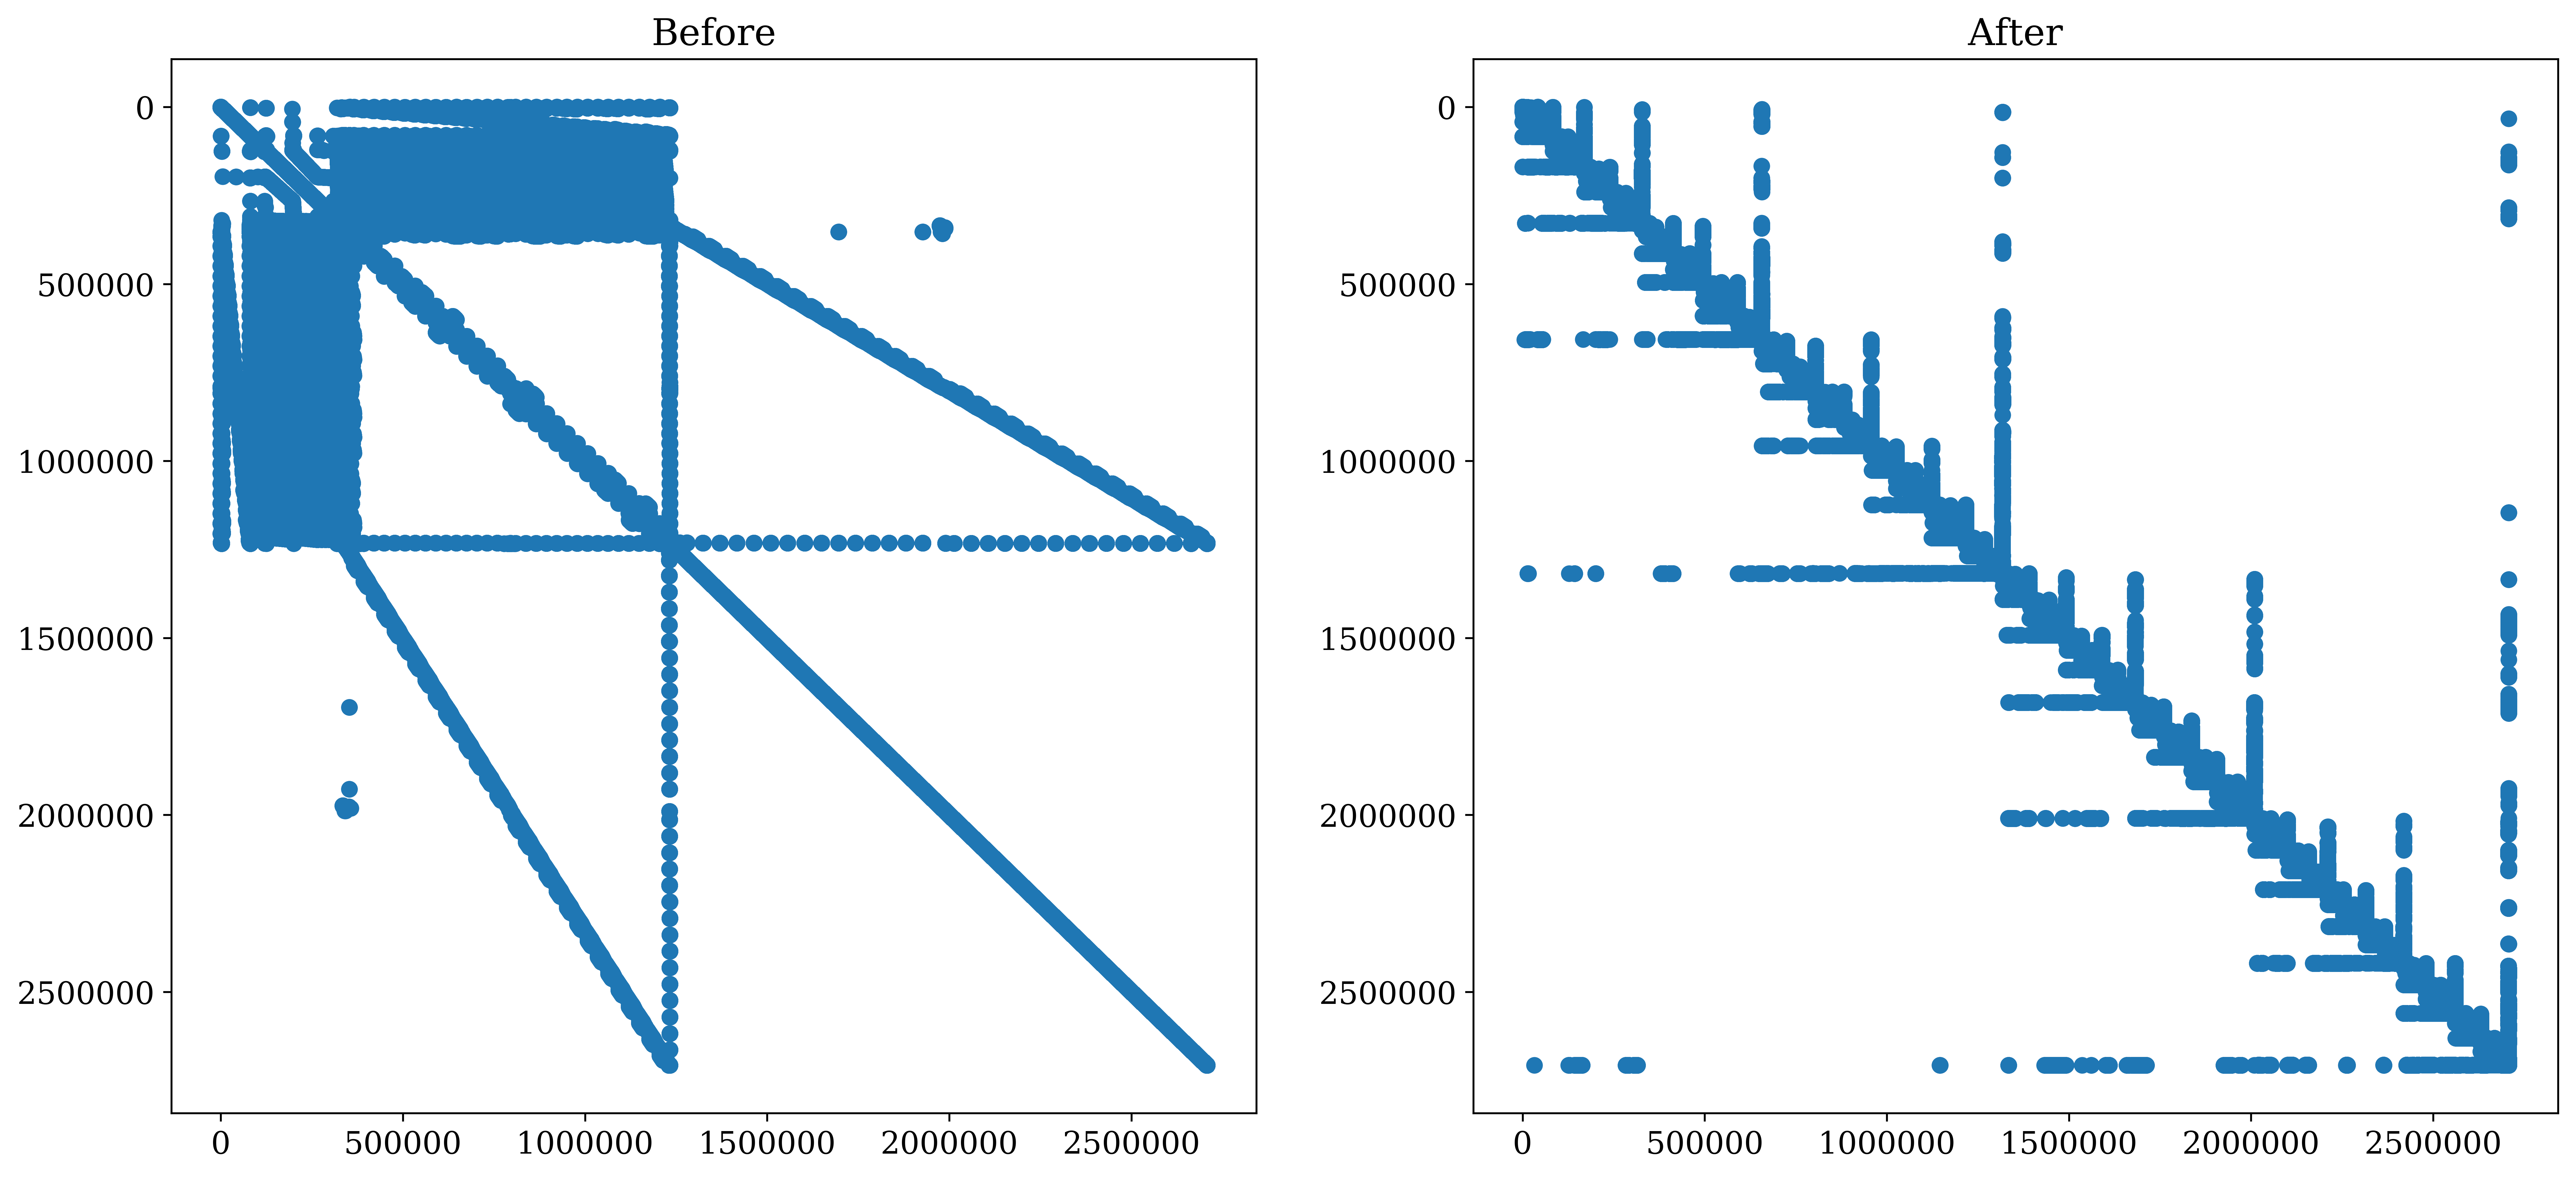
\includegraphics[width=1.00\textwidth]{figures/chapter-2/memchip-matrix-sparsity-pattern.png}
%\caption{Sparsity structure of the matrix \textit{\textbf{memchip}} before and after fill-in reduction}
%\label{fig:memchip-matrix-sparsity-pattern}
%\end{figure}




%As we can see, our model and the experiment show the same trend and the results are pretty much close to each other. However, our model takes into consideration only task parallelism whereas MUMPS exploits both data and task parallelism. Additionally, we have to mention that our model 1 works well only for relatively big sparse matrices. It can be quite inaccurate in case of small/skinny sparse systems. \\


%In general, it is possible to refine our models and make them more accurate, using Bulk Synchronous Parallel (BSP) approach, for example. However, it will require to possess a real postordered elimination tree, extracted from a specific implementation of multifrontal method, together with information about supernodes sizes. We strongly believe the new enhanced model can explain the jagged strong scaling behavior of the MUMPS solver that we can observe in figure \ref{fig:model-1-vs-mumps}. But, this approach seems to be quite cumbersome and requires to delve into the source code of a particular library. It is needless to say that data can be retrieved only during run time and only after the analysis phase. This makes it less valuable and we can see that it is definitely a wrong way to go.\\


%There are few important aspects to discuss at the end of the section. Numerical robustness is the main advantage of the multifrontal method. It does not require any preconditioner to solve a system of equations. As we discussed in the previous section, tuning a specific preconditioning algorithm can take a considerable amount of time, especially in case of our systems. As another advantage, the method (heavily) exploits matrix sparsity which lowers computational complexity up to $O(n^2)$. In case of massively huge matrices, the algorithm can utilize the secondary memory which sometimes is only one way to solve a system.\\


%We can conclude, from the analysis above, the method has inherently bad scaling behavior and it is quite sensitive to a matrix structure. We will see later that it is almost impossible to predict the saturation point i.e. a point after which performance either drops or stays at the same level. We assume that scaling becomes better with growth of a matrix size. However, we cannot expect such behavior for small and medium systems.\\  


%Secondly, we can see the algorithm requires many pre-processing steps to be done before numerical factorization phase. All these steps must run in parallel and be highly scalable. Apart from performance constrains of the steps, they must lead to wide and well balanced elimination trees which becomes crucial during the numerical phase.\\


%Lastly, the algorithm can fail due to incorrect  working space prediction. As a results, factorization has to be restarted with some modification of input solver parameters.\\



\subsubsection{Threshold Pivoting and Solution Refinement}
\label{subseq:pivot-hadling}


Because of the cumulative effect of inexact computer arithmetics due to a floating point representation of real numbers and, as a result, truncations and rounding errors, small numerical values along the matrix main diagonal can result in significant numerical inaccuracy of the Gaussian Elimination process. Therefore, partial pivoting is a crucial step of Gaussian Elimination. It implies to interchange rows and columns of a matrix in such a way to place distinct and distant values form zero to the main diagonal.\\


In case of direct dense methods, partial pivoting is a straightforward operation and can be expressed as multiplication of the original matrix $A$ by a permutation matrix $P$, where each row and column contain a single $1$, at the corresponding place, and $0$s everywhere. However, it becomes a problem when it deals with direct sparse methods.\\


On the one hand absence of numerical information during the analysis phase makes it impossible to perform partial pivoting at this step. On the other hand application of partial pivoting during numerical factorization usually distorts all matrix re-orderings and, therefore, the elimination tree structure. As a consequence, partial pivoting can lead to significant fill-in, load unbalance and, as a result, slow-down of numerical factorization. For that reason, threshold pivoting is used, in practice, instead of partial pivoting.\\


Threshold pivoting means that a pivot $|a_{i,i}|$ is accepted if it satisfies equation \ref{eq:lc-1}.\\
\begin{equation}\label{eq:lc-1}
|a_{i,i}| \geq \alpha \times max_{k=i \dots n} |a_{k,i}|
\end{equation}

where $\alpha \in [0,1]$ and $k=i \dots n$ represents row indices of column $i$ within a frontal matrix.\\

Factorization of a column is suspended i.e. delayed, if equation \ref{eq:lc-1} cannot be satisfied within a fully-summed block of a frontal matrix. In this case, the column and the corresponding row are moved to the parent frontal matrix as a part its contribution block where the process repeats again. The process is also known as delayed pivoting and helps to improve numerical accuracy. Higher values of $\alpha$ leads to more accurate solutions but often generate extra fill-in and lead to load unbalance which, as a result, affect parallel performance. On the other hand, smaller values usually preserve the original elimination tree and, therefore,  keep load balance computed during the analysis phase by appropriate mapping of processors across nodes of the tree. However, in this case, numerical accuracy usually degrades. In practice, values of $\alpha$ lay in a range of $0.2$ to $0.04$ \todo{REF}.\\



A case when parameter $\alpha$ is equal to $0$ is known as static pivoting which means that no pivoting is performed during the numerical factorization phase. This allows to better optimize data layout, load balancing, and communication scheduling \cite{superlu-manual} before numerical factorization which is supposed to improve parallel performance.\\



By and large, solutions computed by direct sparse methods are usually numerically inaccurate, in some degree, and often demands to perform solution refinement. As an example, solution accuracy can be improved using the iterative refinement method. Code listing \ref{lst:iterative-refinement} shows a psedu-code of the method where parameter $\omega$ represents an estimation of the backward error, equation \ref{eq:backward-error}, \cite{mm-backward-error}. In practice, the method usually takes 2 or 4 iterations to achieve sufficient numerical accuracy.\\

\begin{equation} \label{eq:backward-error}
\frac{|b - A\hat{x}|_{i}}{(|b| + |A| |\hat{x}|)_{i}}
\end{equation}

where $\hat{x}$ is the computed solution; $|\bullet|$ is the element-wise module operation.\\


\begin{minipage}{\linewidth}

\begin{lstlisting}[language=python, caption={Iterative refinement}, frame=single, label={lst:iterative-refinement}]
# perform analysis and numerical factorization  phases
LU = SparseDirectSolver(matrix=A)

# compute initial solution
x = Solve(factorization=LU, rhs=b)

# compute initial residual
r = A * x - b

while r > $\omega$
	# find correction
	d = Solve(factorization=LU, rhs=r)
	
	# update solution
	x = x - d
	
	# update residual
	r = A * x - b
\end{lstlisting}
\end{minipage}


As an alternative to the iterative refinement method, one can use the resulting $LU$ decomposition of matrix $A$ as a preconditioner for an iterative solver, for instance GMRES. The practice, in particular of ATHLET users, has been shown that it usually takes 1 \dots 3 iterations to achieve desired numerical accuracy even with extreme small values of $\alpha$.\\

At the end, it is worth mentioning that both refinement techniques, mentioned above, exploit only data-based parallelism and, therefore, scale well on distributed-memory machines.\\